\documentclass{article}

\usepackage{color}
\usepackage[margin=1in]{geometry}
\usepackage{graphicx}
\usepackage{hyperref}
\usepackage{listings}

\definecolor{gray}{rgb}{0.5, 0.5, 0.5}
\definecolor{darkgreen}{rgb}{0, 0.6, 0}

\begin{document}
    \raggedright
    Homework 5 \break
    Christopher Seagraves
% % % % % % % % % % % % % % % % % % % % % % % % % % % % % % % % % % % % % % % % 

    \section*{Problem 1}
    \url{https://github.com/nosv1/seagraves_unmanned_systems/tree/main/SearchAlgorithms} \break

    \begin{tabular}{|c|c|c|}
        \hline
        & Time & Travel Cost \\
        \hline
        AStar & 0.015 & 49.8 \\
        \hline
        Dijkstra & 0.017 & 49.8 \\
        \hline
        RRT & 20.452 & 75.58 \\
        \hline
    \end{tabular} \break
    \begin{center}
        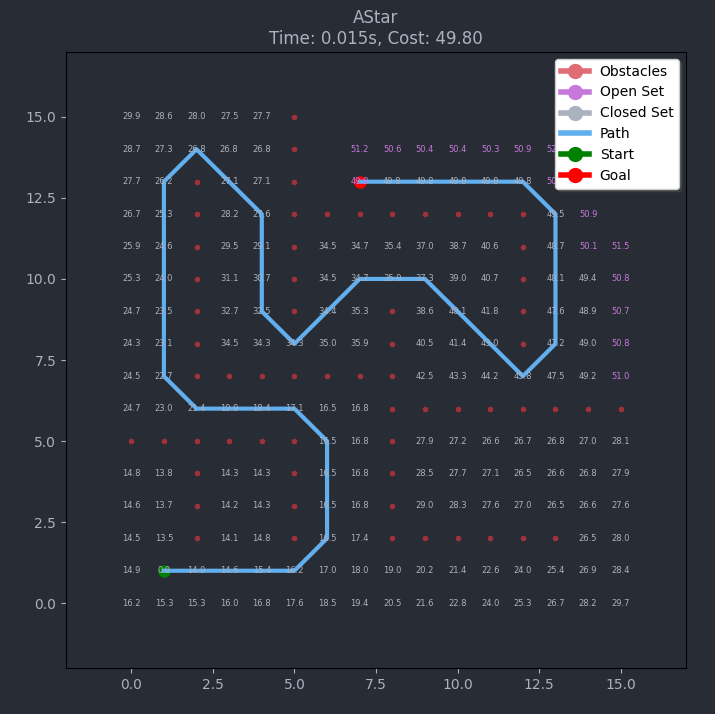
\includegraphics[width=3in]{AStar.png}
        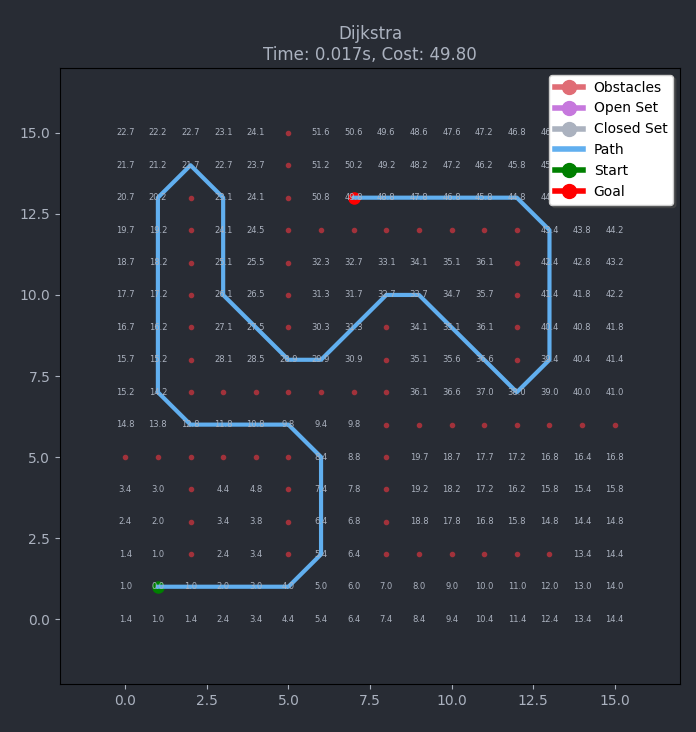
\includegraphics[width=3in]{Dijkstra.png} 
        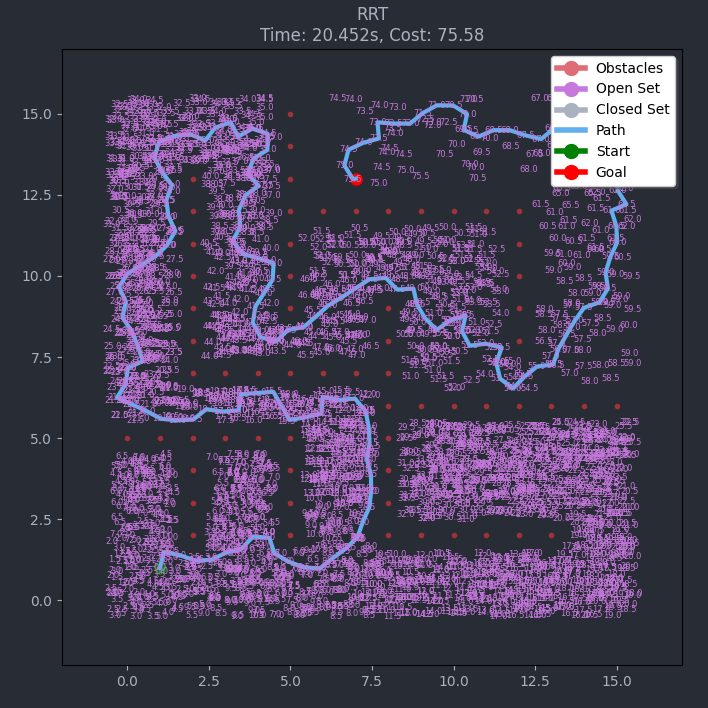
\includegraphics[width=3in]{RRT.png}
    \end{center}
    \raggedright
    Yes, this is what I expected in terms of times and costs. AStar on a 'complex' map compard with Dijkstra will complete at similar times, and find the most effiient paths. However, RRT is still terrible on small maps in terms of time and cost.
        
% % % % % % % % % % % % % % % % % % % % % % % % % % % % % % % % % % % % % % % % 
    \section*{Problem 2}
    \raggedright
    \url{https://github.com/nosv1/seagraves_unmanned_systems_pkg/blob/master/seagraves_unmanned_systems_pkg/PathFollower/path_follower.py} \break

    The graphs below demonstrate a turtlebot set with a Vmax of 0.95 m/s and max turn-rate of 2.84 rad/s. The turtlebot was tuned with a heading\_pid and a throttle\_pid. \break
    Heading PID: Kp=4.5, Ki=0, Kd=0.25 \break
    Throttle PID: Kp=0.4, Ki=0, Kd=0.02
    \begin{center}
        AStar
        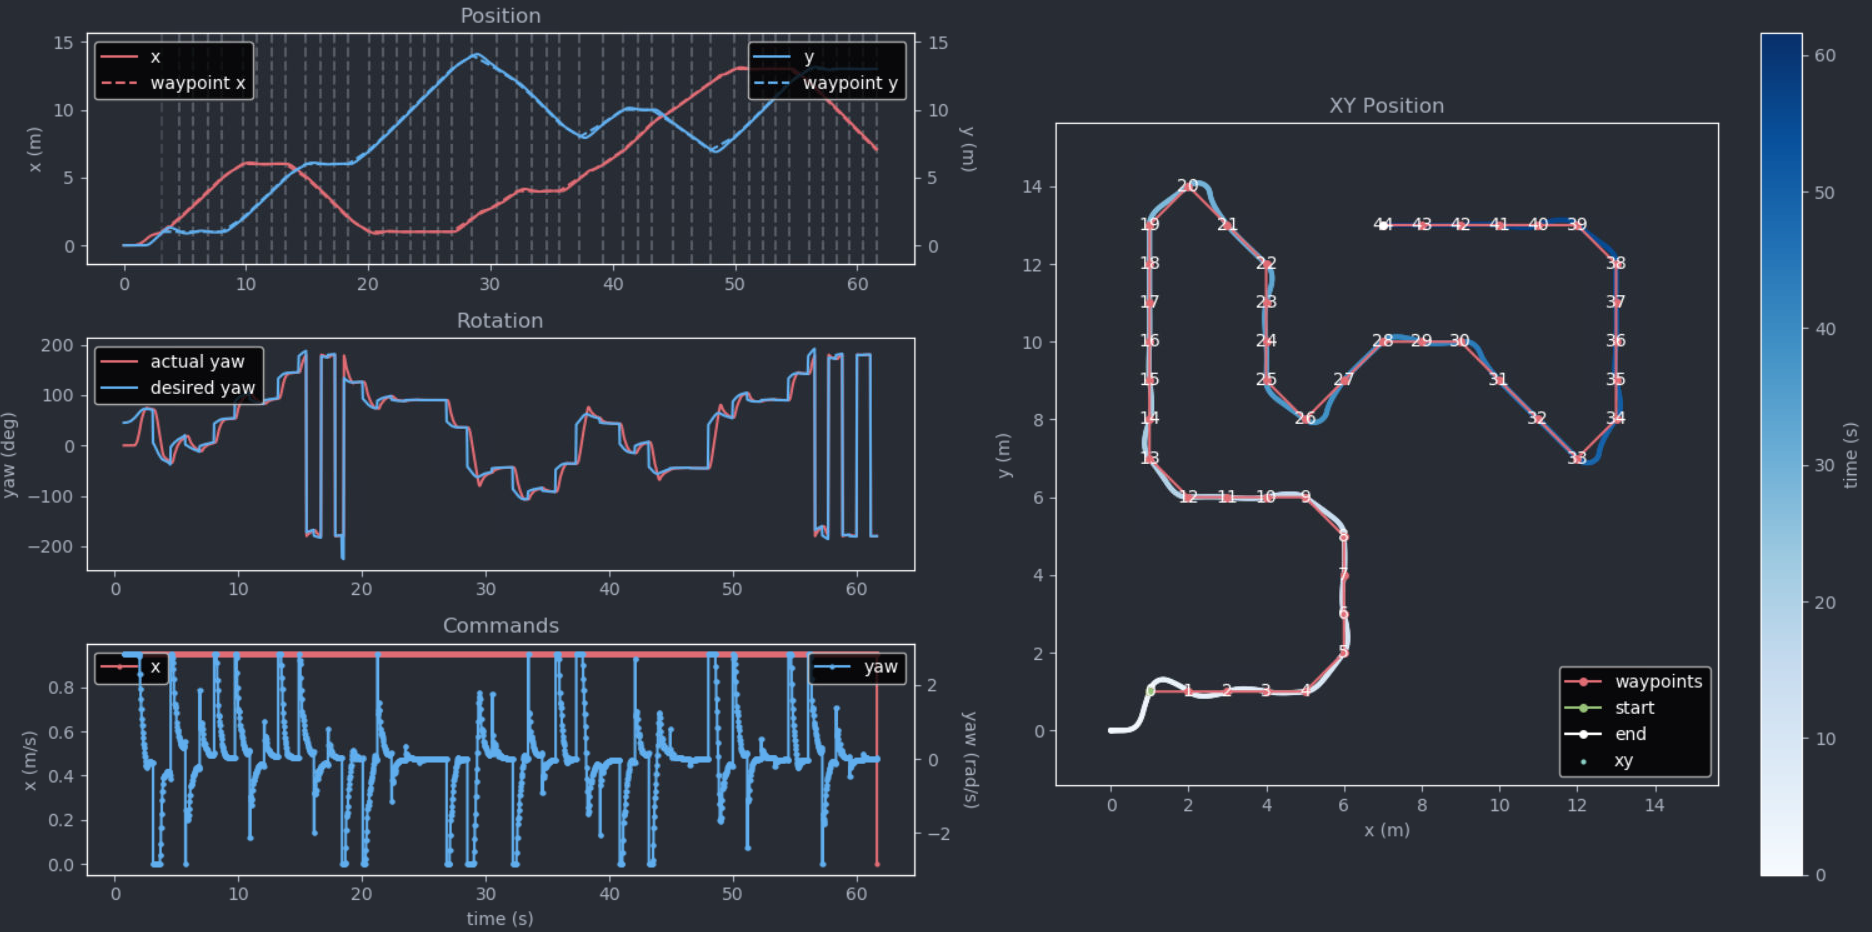
\includegraphics[width=\linewidth]{AStar Turtlebot.png} \break

        RRT
        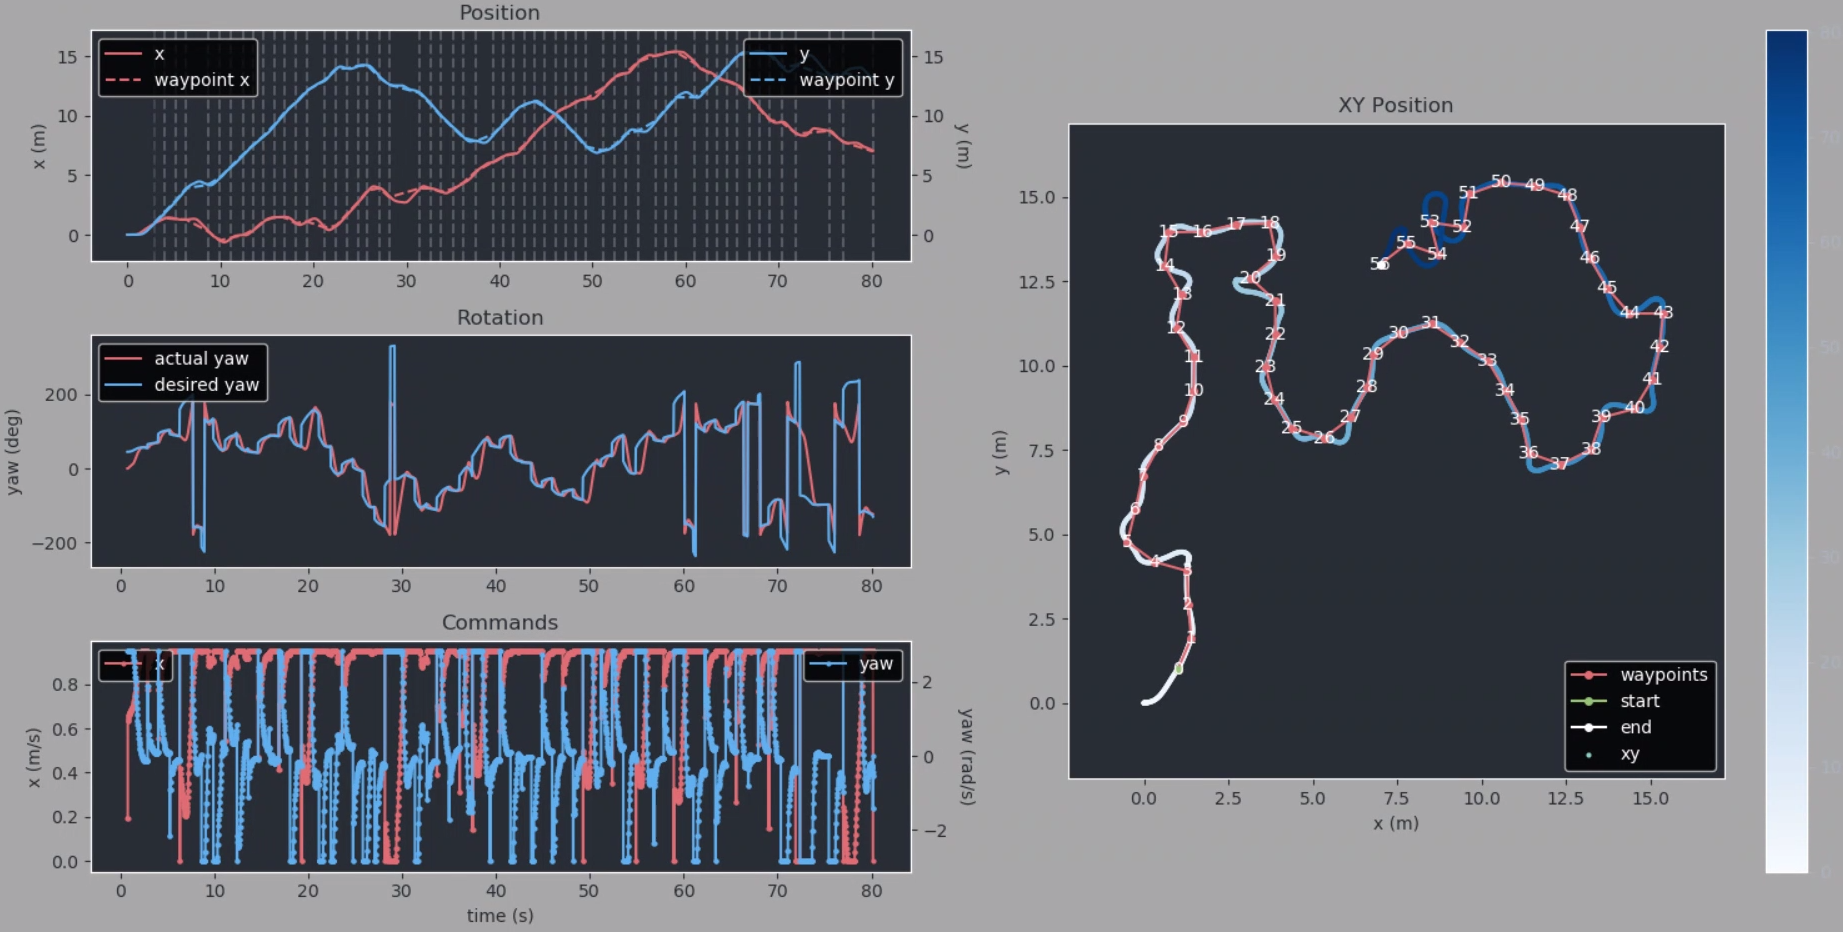
\includegraphics[width=\linewidth]{RRT Turtlebot.png}
    \end{center}
        
% % % % % % % % % % % % % % % % % % % % % % % % % % % % % % % % % % % % % % % % 
    \section*{Problem 3}
    \url{https://github.com/nosv1/seagraves_unmanned_systems/blob/main/HW5/TSP_main.py}\break

    \begin{center}
        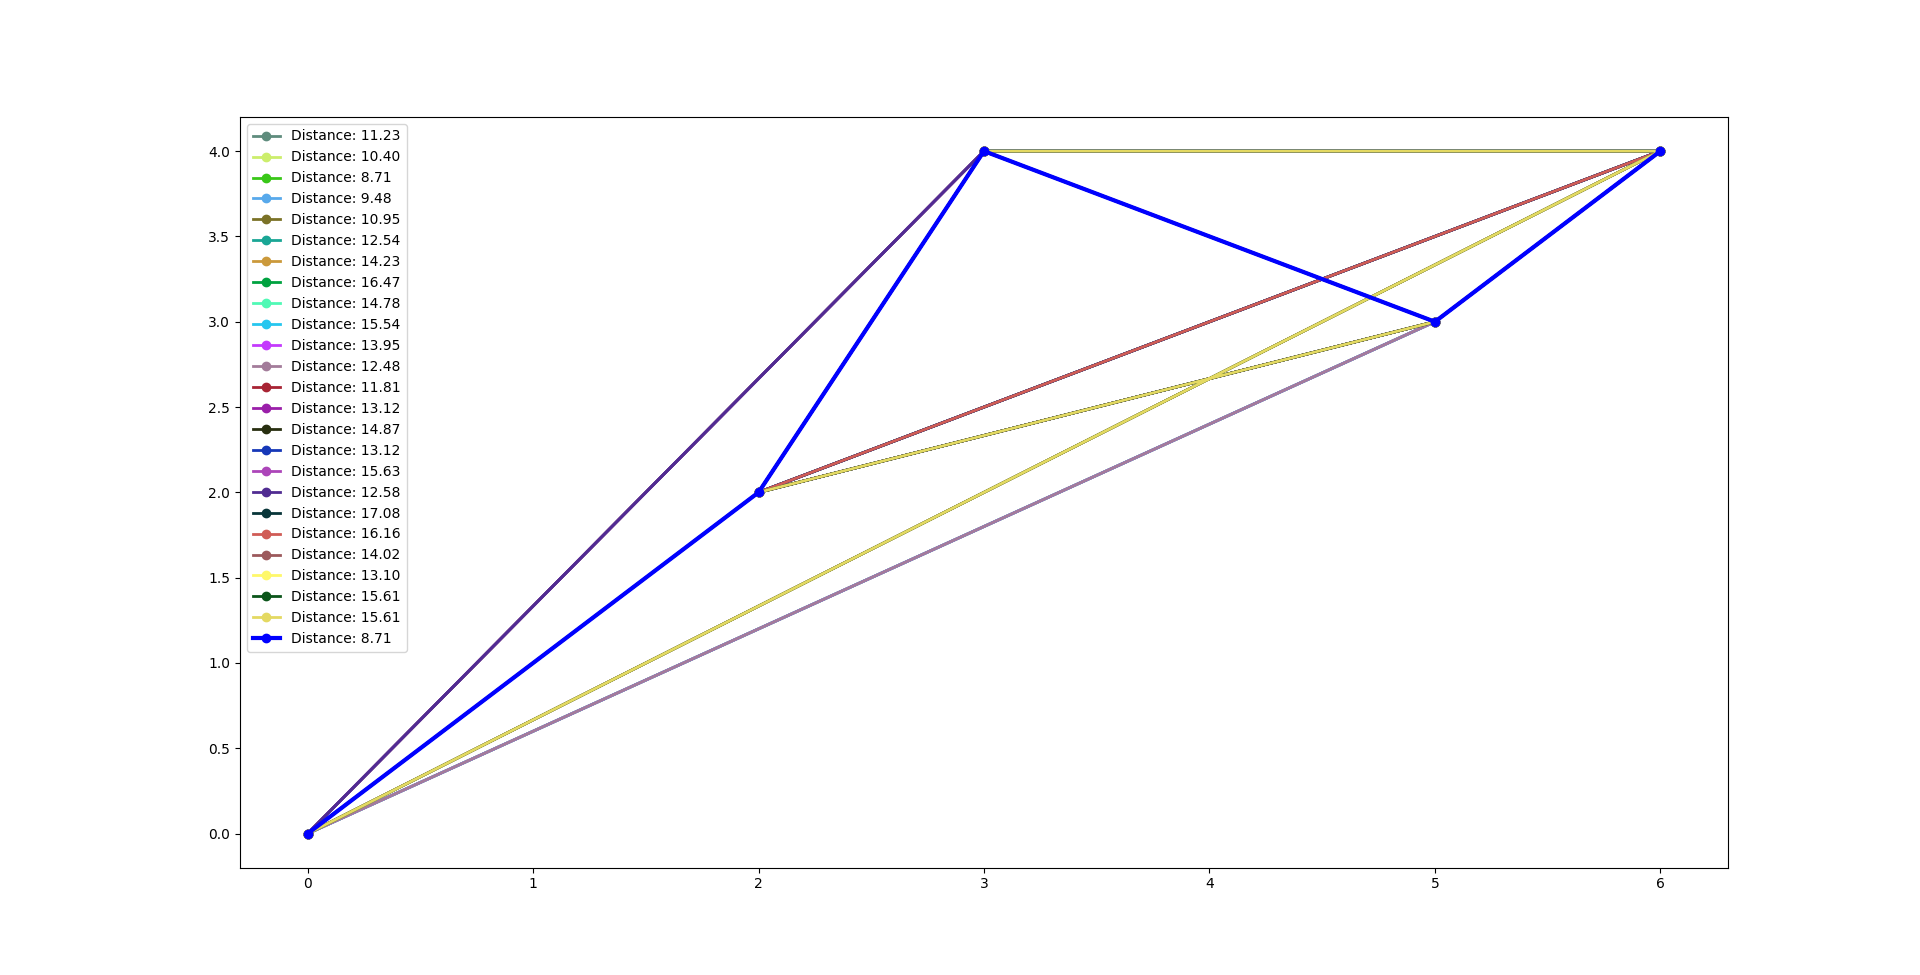
\includegraphics[width=3in]{TSP.png}
    \end{center}

    \raggedright
    For fun, I tried to generate a more complicated path, but seemed 11 points + start was my PC's limit... Even parellizing what I could, 40 million combinations (11!) is a doozy.
    Given we had a non-moving start point though, a trick was to generate all the paths that don't include start, then just add the distance from start and the first point in the permutation when you calculate the distances. 

    \begin{center}
        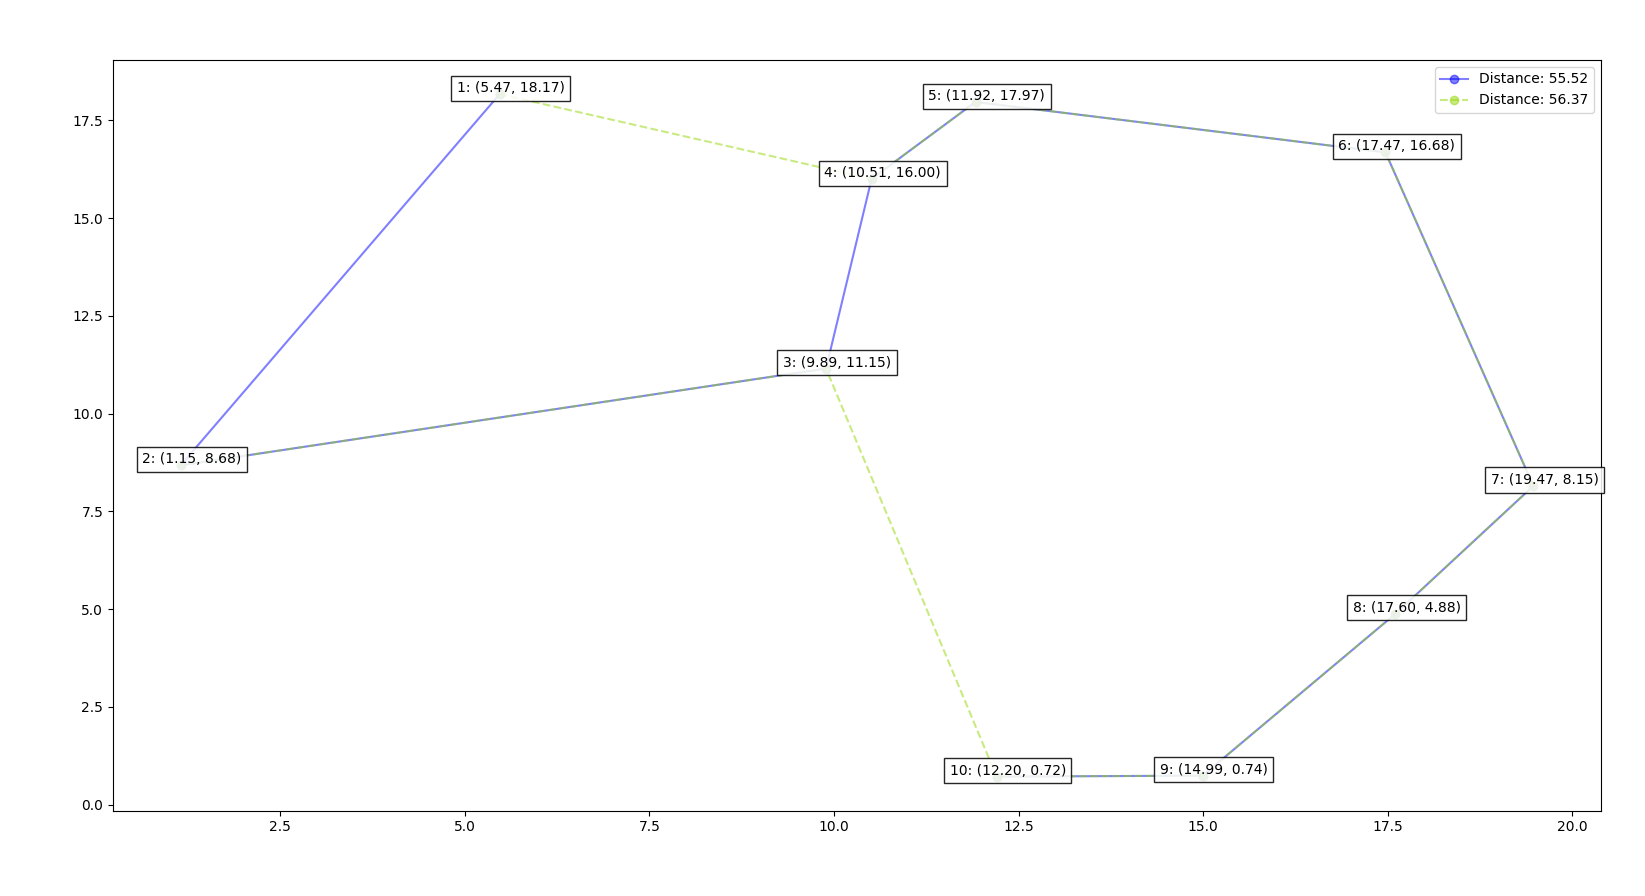
\includegraphics[width=5in]{TSP 11 points.png} \break
        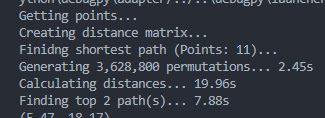
\includegraphics[width=3in]{TSP 11 points console.png} \break

        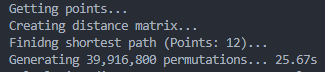
\includegraphics[width=3in]{TSP 12 points console.png} \break
        Calculating distances never completes...
    \end{center}
        
% % % % % % % % % % % % % % % % % % % % % % % % % % % % % % % % % % % % % % % % 
\end{document}